\chapter{Theoretical background}
\label{chapter:background}

In this chapter, I introduce the necessary theoretical background. Unless specified otherwise,
the material presented in this chapter is based on the textbook on distributed algorithms by Hirvonen and Suomela~\cite{Hirvonen2020}.

\section{Graphs}

This section will outline the necessary theoretical background on graphs. 
Most of the notation related to the graph theoretic concepts in the current
section and the rest of the thesis will follow that of
the recent introductory textbook on distributed algorithms~\cite{Hirvonen2020}
unless specified otherwise.

A \emph{graph} is a pair $G = (V, E)$, where $V$ denotes the set of all \emph{vertices}
and $E$ denotes a set of all \emph{edges}. Each edge in $E$ is represented as a set of
2 nodes i.e.\ the nodes the given edge is connecting e.g.\ $e = \{v, u\}$ such that 
$v \in V$ and $u \in V$.

When talking about the \emph{size of a graph}, or \emph{cardinality} of the graph, I refer
to the number of nodes in the graph. Or in other words, the size of a graph $G$
is always $|V|$.

Among other things, edges can be categorised into \emph{directed} and \emph{undirected}.
The latter ones simply connect a pair of nodes in a graph, while the latter
ones also contain extra information about which of the two connected nodes is
a ``source'' and which one is a ``destination''. Informally, such a directed edge
can be visualised as an arrow that starts in a ``source'' node and ends in a 
``destination'' node.  Similarly, we talk about \emph{undirected graphs} -- that is, graphs
where all edges are undirected, and \emph{directed graphs} -- such graphs where all
edges are directed. Formally, while an undirected edge $e$ is defined as a
set of two nodes $e = \{v, u\}$, a directed edge $e$ is defined as a pair
of two nodes $e = (v, u)$. Recall that in the case of a pair, the order of its
elements does matter, hence, the pair allows us to encode the direction of
the edge. Unless mentioned otherwise, we assume that an edge is directed
from the first element of the pair to the second. Also note that in this
thesis, unless specified explicitly, all graphs are assumed to be undirected.

If two nodes are connected by an edge, we call such nodes \emph{neighbors}. We
also say that such nodes are \emph{adjacent} to each other. Moreover, in an undirected graph
if there are two edges $e_1$ and $e_2$ such that $e_1 \neq e_2$ and $e_1 \cap e_2 \neq \emptyset$
such edges are said to be \emph{adjacent} to each other. Similarly, we can talk about adjacent 
edges in a directed graph. In that case, two edges $e_1$ and $e_2$ are adjacent if
$e_1 \neq e_2$ and either first or second element of the pair $e_1$ contains the same
element as either first or second element of the pair $e_2$.

Besides, we often talk about edges and nodes being \emph{incident} to each other.
In an undirected graph, an edge $e$ is incident to a node $v$ if and only if $v \in e$. In this
case, we also say that the node $v$ is incident to the edge $e$. Similarly, in a
directed graph, an edge $e$ is incident to a node $v$ if and only if $v$ is the
first or the second element of the pair $e$. Again, in the case described in the
previous sentence, the node $v$ is said to be incident to the edge $e$.

We also often talk about \emph{ports}. A port can be thought of as an end
of an edge $e$ associated with a node $v$ so that $e$ is an incident edge
of $v$. Therefore, each edge $e = \{v, u\}$ has two ports associated
with it. One port belongs to node $v$, and another port belongs to
node $u$. From this, it follows that each node has as many ports
as it has incident edges.

A \emph{simple graph} is an undirected graph where no two nodes are connected by more
than one edge and no edge starts and ends at the same node. In other words, there are
no multiple edges or self-loops in a simple graph.

A \emph{degree} of a node $v \in V$ in a graph $G = (V, E)$ is the number of all
edges incident to $v$. That is, it is the number of edges such that for an edge
$e$, $v \in e$ if $e$ is an undirected edge, or $v$ is the first or second element of
pair $e$ if $e$ is a directed edge. Moreover, for directed graphs, we often talk
about \emph{indegrees} and \emph{outdegrees}. Indegree of a node $v$ is the number
of edges incident to $v$ directed towards the node, while outdegree of a node $v$ is the 
number of edges incident to $v$ directed outwards from the node. Finally, we are 
often interested in a maximum degree of a graph $G$, that is, the maximum value of
degrees of all nodes belonging to the graph $G$. I denote such maximum degree as
$\Delta$. In this work, we only consider graphs whose nodes' degrees
are bounded by a constant. That is, the degree of each node is
necessarily finite and does not depend on the size of the graph.

A \emph{walk} in an undirected graph $G = (V, E)$ is a sequence $w$ of a form
$w = (v_0, e_1, v_1, e_2, ..., e_l, v_l)$,
where $v_i \in V$ and $e_i \in E$, and $e_i = {v_{i-1}, v_i}$ for all $i$. A walk from some
node $v$ to some other node $u$ is then a walk $w$ such that its first element i.e.\ $v_0 = v$
and its last element i.e.\ $v_l = u$. Having defined a walk, we can talk about a \emph{
connected graph}. A connected graph, when talking about undirected
graphs, is a graph $G = (V, E)$ in which for any pair of nodes $v$ and $u$ such that
$v \neq u$ there is a walk from $v$ to $u$. In this work, all the graphs
should be assumed to be connected unless specified otherwise.

An \emph{isomorphism} between two graphs $G_1$ and $G_2$ is a function $f$ such that $f$ is a 
bijection, and $f$ maps a vertex of the graph $G_1$ to a vertex of the graph $G_2$, and 
an edge between some nodes $v$ and $u$ exists in the graph $G_1$ if and only if
an edge between nodes $f(v)$ and $f(u)$ exists in the graph $G_2$. From this,
it is rather easy to see that if an isomorphism exists from $G_1$ to $G_2$, then
also an isomorphism exists from $G_2$ to $G_1$. If there exists an
isomorphism between some two graphs, we say that such graphs are isomorphic
(to each other).

A \emph{radius-x neighborhood} of a node $v$ in a graph $G = (V, E)$ is a set of
all such nodes $u \in V$ that there exists a walk between $v$ and $u$ and 
the shortest walk from $v$ to $u$ is at most $x$. Note that it is possible that
$v = u$, in which case the shortest walk between $v$ and $u$ is 0.

A diameter of a graph (denoted as $\diam(G)$) is the length of the longest walk
in a list $W$, where $W$ is a list of the shortest walks, i.e.\ the one between each pair of nodes
$v$ and $u$ in a graph $G = (V, E)$ such that $v \in V$ and $u \in V$. If a graph
$G$ is not connected and, therefore, there is a pair of nodes $v$ and $u$ that does not
have a walk between them, we say that a diameter of such a graph $G$ is infinity. That
is, $\diam(G) = \infty$.

\subsection{Several important graph families}

This subsection will introduce some of the graph families that will be necessary
for understanding the content of the thesis. First, I will define paths and cycles.
Then, I will briefly introduce trees and explain the difference between rooted
and unrooted trees.

A \emph{path} graph is a sequence of nodes that are joined together by edges and
have the following properties:

\begin{enumerate}
  \item The whole graph is connected. That is, there is a walk from any node of
  the path to any other node of the path.

  \item The graph consists of at least two nodes.

  \item Exactly two nodes have a degree 1, and all the other nodes have a degree~2.
\end{enumerate}

A \emph{cycle} is a connected graph where each node has a degree 2.
If a graph $G$ is a cycle or by removing several nodes and/or edges
from the graph $G$ we can obtain a cycle graph, then we say that
$G$ contains a cycle. On the other hand, if $G$ is not a cycle, and
it is not possible to obtain a cycle from $G$ just by removing some
nodes and edges from it, we say that such a graph does not contain a
cycle, or that it is acyclic.

A \emph{tree} is an undirected acyclic connected graph. A \emph{rooted tree}
has a single \emph{root vertex}, and thus some nodes have a \emph{parent} node
(some because e.g.\ a root node never has a parent) and one or more \emph{children}
nodes. For a node $v$, a node $u$ is its parent if and only if $v$ and $u$ are
neighbor nodes, and the shortest walk from the root to $u$ is shorter by exactly
1 compared to the shortest walk from the root to $v$. Node $v$ is a child of node
$u$ if and only if $u$ is a parent of node $v$. Finally, in the context of rooted trees,
a node $l$ that has no children is referred to as a \emph{leaf} node.
On the other hand, an \emph{unrooted tree} has no single root, and therefore the notion of parent
or child is not defined. Instead, we talk about neighbors of some node $v$. However, we 
still use the notion of leaves to denote nodes of degree 1.

\subsection{Biregular trees}
\label{subsection:biregular-trees}

A \emph{bipartite} graph $G = (V, E)$ has its vertices partitioned into two
subset $U \subseteq V$ and $W \subseteq V$ so that the partitioning forms
a proper 2-coloring of the node $V$. In other words, in a bipartite graph $G = (V, E)$,
if a node $v \in U$ then all its neighbors belong to $W$, and if a node $v \in W$
then all its neighbors belong to $U$.

A \emph{regular} graph is a graph where each vertex has the same degree.
A \emph{biregular} graph is a graph where each vertex has one of the two
allowed degrees and only them. In this thesis, when we talk about
\emph{($\beta$, $\delta$)-biregular} graph $G$, we always assume that 
$G = (V, E)$ is bipartite so that $V$ is partitioned into two
subsets $U$ and $W$, nodes of these subsets together form a proper 2-coloring,
all nodes in $U$ are of degree $\beta$, and all nodes in $W$ are of
degree $\delta$. In particular, when I talk about \emph{($\beta$, $\delta$)-biregular trees},
I mean a bipartite biregular tree where all nodes except for the leaves
follow the rules of ($\beta$, $\delta$)-biregular graphs described above,
but leaves themselves are allowed to have degree 1 (otherwise they would not be
called leaves).

It is important to notice the equivalence of ($\delta$, 2)-biregular trees
and $\delta$-regular trees. Indeed, given a $\delta$-regular tree, we can
``turn'' each edge $e = \{v, u\}$ into a node $v_e$ such that the node is
connected to node $v$ and $u$ and only those nodes. On the other hand,
given a ($\delta$, 2)-biregular tree, we can remove every node $v$ of degree
2 and, given that nodes $u$ and $w$ used to be neighbors of $v$ before its
removal from the graph, connect nodes $v$ and $w$ with an edge.

\section{Distributed computing}

Now that I have introduced some of the key graph theoretic concepts, I will
next outline some of the foundations of distributed computing. We will start with
a short historical note about the field of distributed computing. Then, I will
explain some of the aspects of the model of computation we are concerned with. Finally, 
I will give some formal definitions of the model of computation that will be our
major concern throughout the rest of the thesis.

\subsection{General background}

The field of distributed computing studies computation in distributed systems, which
have become ubiquitous in the modern world, being especially prevalent
in the area of technology~\cite{Attiya2004}.
A distributed system consists of a number of relatively independent
computing modules, which usually need to cooperate in order to
fulfill a computational task the system has been given. Usually,
each computing module in such a system only has a part of the whole
input and is required to produce only a part of the whole output.
This is in contrast with a centralized system, in which there 
exists an all-knowing entity taking all of the input, performing all
of the computation, and producing the whole of a result as its output.
Due to its modularised and parallel nature, distributed computing
has many applications in communication, computation, the Internet,
but also in biology and sociology~\cite{Wattenhofer2016}.

The field of distributed computing appeared already in the late 1980s, with several
prominent papers exploring potentialities of computation performed
by multiple interconnected processing units~\cite{Cole1986, Linial1987, Naor1991}.
The first major step in the field happened in 1987 when Linial formalized
some of the principles of one variant of a distributed system.
This model of computation is currently known as Linial's or the \emph{LOCAL model}~\cite{Linial1987}.

\subsection{Model of computation}

Here, I will describe the model of computation that we are going to
assume throughout the rest of the thesis.
Note that there are several
different models, which are also widely studied
in the research community.

First, as it was already stated, unlike in the case of centralized
computation, we are concerned with multiple interconnected computing entities
that together form a graph. Each such entity is referred to as a vertex or
a node in a graph. Connections between the vertices are referred to as edges.
The entities only can transfer information along the edges and in no other way
between each other. Unless specified otherwise, the graphs are assumed to be
simple graphs, and all edges are assumed to be undirected. Moreover,
communication along the edges can simultaneously happen in both directions.

Apart from sending information to each other, nodes can also
do local computation based on the local information each node possesses. One thing
to note that differs significantly from some of the centralized models of computation
is that each vertex in a graph has arbitrarily huge, but finite, storage and computation resources.
Informally, this means that anything that can be computed in a centralized setting
in a finite amount of time
can also be computed locally by a node in an arbitrarily small amount of time.
It is also worth noticing that in the model of computation described here,
every node of a graph executes the same algorithm. Nevertheless, the
algorithm might lead to different commands being executed by different nodes
if, for example, nodes' unique identifiers or initial local inputs are different.
Besides, the behavior might also differ if two nodes have somewhat different neighborhoods
around themselves and therefore will receive potentially different
information during their communication rounds. Finally, at the beginning of
execution, each node knows only its own input (including its own unique identifier) and its own degree i.e.\ the number of
its neighbors.

Furthermore, computation in a graph happens in synchronous rounds. That implies,
for example, that round $x+1$ is not started by any of the nodes before all of the
nodes have completed round $x$. Each round is divided into three stages:

\begin{enumerate}
\item sending some information to some (or all) of its neighbors,

\item receiving information
from some (or all) of its neighbors,

\item performing some local computation based
on the information that has been stored by a node locally before and the information
received during the current round from its neighbors,

\item updating its local state i.e.\ replacing and adding data in its own local storage.
\end{enumerate}

Each of these stages is also executed
completely synchronously by all nodes in a graph, meaning that e.g.\ no node starts processing
any of its data, before all other nodes have received data from their neighbors. The computation
of a graph is said to be finished when all of the nodes have outputted their final states
and halted. More formally, this means that there are a set of node states that are
considered as \emph{halting states}. Whenever a node switches its internal state to one of the 
halting states, it does not perform any of the actions starting from that point in time, or -- to
be even more formal -- it does not send any messages to its neighbors, ignores all of the 
messages sent to it, and does not update its internal state in all of the subsequent rounds.
In addition to the requirement that the local computation of each node in each round has to be finite
and needs to stop after a finite amount of time passed, all nodes are required to eventually
transition into one of the halting states. That is, a valid distributed algorithm -- in our model of
computing -- cannot continue for an infinite number of rounds. Finally,
the complexity of a distributed algorithm is measured as the number of such synchronous rounds
of computation before the algorithm ends i.e.\ before all nodes transition into one of 
the halting states. Notice that different from a centralized model of computation,
algorithms complexity (or in other words its running time) is not affected by the
amount of local computation on a single node.

Another important thing that has to be mentioned when describing the mode of computation
is that all of the operations within each node as well as inter-vertex
communication are error-free. In other words, all nodes can be assumed to
always act in a fault-free manner, all sent messages can be assumed to never be lost
or undelivered. Therefore, we can always assume that messages sent and received by nodes
are all in accordance with the actual algorithm that is being executed by the nodes
and not a result of an accidental fault or an intentional adversary effort.

\subsection{Distinctive qualities of the LOCAL model}

As was already mentioned previously, our model of computation is known
as Linial's or the LOCAL model~\cite{Linial1987}. Therefore, to complete the
description, I will describe in more detail two distinctive qualities of the LOCAL model
from other models of distributed computing: namely unique identifiers and arbitrarily large
bandwidth.

Each node in the LOCAL model is provided with a unique identifier as part of the initial input.
The identifiers are usually assumed to be integer numbers between 1 and $|V|^c$, where
$|V|$ is the number of nodes in the graph and $c$ is some constant. Unless specified, we
assume that such a constant $c$ is not known by the nodes at the beginning of
algorithm execution. Thus, unique identifiers are guaranteed to be positive integer
numbers bounded by a polynomial in the number of nodes, but it is not known -- by the nodes
at the start of algorithm execution -- what is the largest unique identifier in the graph. Moreover,
the identifiers of the node do not necessarily form a continuous range of integers. That is,
if an integer $x$ is used as a unique identifier for some node $v$, it is possible
that an integer $x+1$ is not used as an identifier in the graph. This implies that at
the beginning, nodes do not know what integers have been used for unique identifiers
and what have not been, with the exception of only one integer -- their own identifier.

Another characteristic of the LOCAL model, which also was already mentioned before, is the fact
that nodes can send (and receive) an arbitrarily large (but finite)
amount of bytes of information over a single edge during one round. This fact,
combined with the existence of unique identifiers, renders the model as a rather strong one.
In particular, this implies that a node can send all of its information -- no matter how
large it is -- to all its neighbors in just one round.

This, in turn, implies a rather
curious property. Imagine that every node sends all of its information during the first round
and, having received some data from its neighbors, saves all this information locally. Consider
some node $v$ in the middle of a graph $G = (V, E)$. Since all nodes send all their data,
after the first round, node $v$
will have all the data that all its neighbors had initially, plus its own initial information.
Notice that each of $v$'s neighbors now has all the information of their neighbors. Thus,
if we combine all the data in the possession of $v$ and $v$'s neighbors after the first round, it
is easy to observe that they together have all the information of $v$'s radius-2 neighborhood.
But this means that after the second round, when all $v$'s neighbors have sent all their
information to $v$, the node $v$ alone possesses all the data that its radius-2 neighborhood had at the
beginning of the algorithm execution. Similarly, after the 3rd round, $v$ will have all the
radius-3 neighborhood's data, and so on.
In general, after round $x$, node $v$ will have
all information that was initially available in its radius-$x$ neighborhood.
Therefore, when considering the LOCAL model,
time and space are in a certain sense equivalent. In other words, the number of rounds
needed to solve a certain problem is always equal to the distance (or radius) to which a node needs to
see to solve a certain problem. One technicality to note here is that because all nodes have
unique identifiers, and these identifiers are sent together with the rest of the data,
receiving nodes can differentiate what nodes the received data belongs to, and consequently,
reconstruct the structure of the neighborhood in the graph.

As a consequence of the above,
we can observe that after $\diam(G)$ rounds, node $v$ will have all the information there is in the 
graph $G$. This implies that after $\diam(G)$ rounds, in the LOCAL model, we can solve anything that can
be solved in a centralized setting. That is, because at the end of $\diam(G)$'th round, each node in the
graph has collected all the information there is in the graph and thus can just run the
computation locally. And because local computation in the LOCAL model is virtually free,
anything that could be computed in a centralized setting will be computed locally by each
node individually. Then, in the next round, each node can output its part of the solution.

\subsection{Formalizing the LOCAL model}

In this subsection, I will formalize the LOCAL model that I informally described above.
This will, first of all, help to clarify the aspects of the model that are still left ambiguous
after reading the previous subsections. Besides, it will allow us to introduce
a randomized model below once the basic deterministic one is unambiguously defined.

An algorithm being executed by each node consists of 
three functions. One for local state initialization, which is executed only once, after
a node $v$ has received its initial local inputs $u(v)$ but before the first round:
$$\init_A(u(v), d)$$,
where $A$ is a given distributed algorithm and $d$ is the degree of the node $v$.
The function returns an initial local state of the node $v$.

The second function takes as an input an internal state $x(v)$ of a node $v$
and returns a tuple of size $d$, where $d$ is a degree of node $v$. The
tuple contains messages that are to be sent to $d$ neighbors of the node $v$
during the current round.
$$\send_A(x(v), d)$$
The third function takes as an input a local internal state $x(v)$ of a node
$v$, and a tuple $m(v)$ of size $d$ that contains messages received from $d$ neighbors
of the node $v$.
$$\receive_A(x(v), m(v), d)$$
The function returns a new local internal state of the node $v$, which becomes a
starting internal state $x(v)$ in the next round.

\subsection{Randomized algorithms}

This subsection will introduce the randomized distributed model of computation
and highlight some of the differences between randomized and deterministic
models. In this section, the focus will be specifically on the randomized LOCAL
model as opposed to some other distributed algorithms models.

In the randomized LOCAL model, there are two major differences from the
deterministic LOCAL model. First, the function $\init_A(u(v), d)$ becomes
randomised. This means that the initial state $x_0(v) = \init_A(u(v), d)$ of a node $v$ is
chosen from a discrete probability distribution of all possible initial states.
Second, the function $\receive_A(x(v), m(v), d)$ becomes randomised. This means that,
after all messages have been sent and received for round $i$, a new local internal
state $x_i(v) = \receive_A(x(v), m(v), d)$ for a node $v$ is selected from a
discrete probability distribution. Everything else in the model remains exactly
as it is in the deterministic case, that is, no changes are made to the $\send_A(x(v), d)$
function.

Since probabilities are involved when in the randomized setting, it might not be
obvious what it means to ``solve'' a problem. The major problem is that
since states of the nodes are chosen from a discrete probability distribution,
there is always a probability that the output of the nodes will not be valid.
Therefore, there is often a probability that the problem has not been solved
after a certain number of rounds.

But before I define what it means to solve a problem in the randomized setting, it is
worth noting that there exist two kinds of randomized algorithms: ``Monte Carlo'' and
``Las Vegas''. \emph{Monte Carlo} algorithms always stop after a specified $f(n)$
number of rounds, where $n$ is the number of nodes in the graph, but
it is not guaranteed that the output will be a valid one. Monte Carlo algorithms
only guarantee their execution time and succeed only with probability $p$.
\emph{Las Vegas} algorithms, on the other hand, always produce correct output,
once all the nodes in a graph have stopped, but the algorithm will stop after a
specified $f(n)$ number of rounds only with some probability $p$. Thus, in some
way, these types of randomized algorithms are complements of each other:
one guarantees the correctness of the output but has a chance of going over some
specified execution time, while another has a guarantee on the execution time
but has some probability of producing incorrect output. In the rest of the thesis,
unless explicitly specified otherwise, we can assume that the randomized algorithms
are Monte Carlo algorithms.

Finally, I now can define what it means to solve a problem in a randomized context.
When saying that a certain randomized algorithm ``solves'' a certain problem in
$T(n)$ rounds, unless specified otherwise, I mean that the algorithm stops after
$T(n)$ computational rounds, and the nodes output (or to be more precise the nodes
have transitioned to one of the output states) a correct solution ``with high
probability'' (often denoted as ``w.h.p.''). Formally, if an algorithm succeeds with
high probability, it means that the algorithm succeeds with the probability of at least
$1 - 1 / n^c$, where $n$ is a number of nodes in a graph and $c$ is some constant
such that $c > 0$. Moreover, $c$ is a constant that can be freely chosen when 
running the algorithm. To give a simple example, an algorithm's running time may
linearly depend on such a constant $c$, then before an algorithm is executed,
one may freely choose the constant so that the larger the constant the longer is
the running time, but also the lower the chance that the produced output will
be incorrect. Notice that $c$ does not need to affect running time, but it often
does since the larger it is the lower is the probability of the algorithm's failure,
and decreasing such probability usually comes at the cost of something else -- 
often running time. Thus, when saying that something succeeds ``with high probability''
I do not mean it vaguely but rather refer to a very precise mathematical definition
given above.

\section{Iterated logarithm}

This section will introduce the iterated logarithm function. The function is
one of the most common complexity results of distributed algorithms and will
appear often in the rest of the document.

The iterated logarithm function, denoted as $\log^*(x)$ is defined as follows:
\[
    \log^*(x) = \begin{cases}
        0 & \text{ if $x \le 1$}, \\
        1 + \log^*(\log_2 x) & \text{ otherwise}.
    \end{cases}
\]
The function is notable for the fact that it grows extremely slow. For example,
\begin{align*}
  &\log^*(1) = 0, \\
  &\log^*(2) = 1, \\
  &\log^*(4) = 2, \\
  &\log^*(16) = 3, \\
  &\log^*(65536) = 4, \\
  &\log^*(2^{65536}) = 5.
\end{align*}

\section{Locally checkable labeling problems}

This section will introduce locally checkable labeling problems (from now on referred to as
LCLs), which are the main focus of this thesis. The section will start with
a short historical note and then provide a formal definition of
LCL problems.

As the field of distributed algorithms started to develop, it became clear
that some classes of problems
are of particular interest to the theoretical research community.
One class of such problems has been first introduced in 1993 by
Moni Naor and Larry Stockmeyer under the name of locally checkable 
labeling (LCL) problems~\cite{Naor1993}.

In short, an LCL problem is a distributed problem that satisfies the 
following criteria~\cite{Naor1993, Suomela2020}:

\begin{itemize}

\item The maximum degree of a graph is a finite number that does not depend on $n$.

\item There is a finite number of input labels, and the number is not dependent on $n$.

\item There is a finite number of output labels, and the number does not depend on $n$.

\item The correctness of a solution can be checked locally by each individual node. That is,
after a solution is produced and all the nodes in the graph have stopped, each node can just
check a radius-$O(1)$ neighborhood around itself. The solution is valid if and only if each of
the individual neighborhoods for all the nodes is valid.

\end{itemize}
In the list above, $n$ is the number of nodes in the graph. Finally, as is easy to see from the definition of LCL
problems
above, there is always a finite representation of any LCL problem. Indeed, one can simply list
all valid local neighborhoods, list all valid input labels, list all valid output
labels, and specify the maximum degree of a graph. Since all of the beforementioned are
of size $O(1)$, it is always possible to have a finite representation of an LCL.
In practice, however, in many cases, it is more practical to come up with
a more concise representation. We will return to the topic of representing LCL
problems later in this thesis.

The study of LCL problems has been one of the major research directions
during the last 6--7 years, with numerous papers published in major
distributed computing conferences
~\cite{Balliu2016, Chang2016, Brandt2017, Chang2017, Fischer2017a, Rozhon2019, Balliu2020-1, Balliu2020-2}.
Currently, the study of LCL problems has reached the stage of maturity with,
for example, the complexity landscape of LCL problems being
almost entirely understood~\cite{Suomela2020, Chang2020a}.

\section{Major LCL problems}

This section will introduce some of the common LCL problems
widely studied in the distributed algorithms research community.
Note that all of the problems also exist in the context of 
centralized computing.

\textbf{Vertex coloring} is perhaps one of the most well-known
problems on graphs. Informally, the goal is to color a graph
in such a way that no two adjacent nodes are colored with the
same color. It is also easy to see that the problem is an
LCL problem because it is sufficient and necessary for each node to check
its radius-1 neighborhood. If each node's radius-1 neighborhood is
a valid one i.e.\ none of the neighbors of node $v$ have the same color as $v$
itself, then and only then the output is a valid vertex coloring.
An example of a solved instance of the vertex coloring problem
is presented in Figure~\ref{fig:vertex-coloring}.

Another well-known and widely studied problem on graphs is
\textbf{edge coloring}. Informally, each edge needs to be
colored in such a way that no two adjacent edges are of the same
color. Coloring edges in a graph can still be simulated
with the setting in which only nodes output the labels.
Each node will output a tuple of the size equal to the node's
degree. Each element of a tuple represents a label
that the node outputs on a corresponding incident edge. The problem
is also an LCL problem because after a final output is
produced, each node $v$ will need to check its radius-1
neighborhood to make sure two things are in order:
\begin{enumerate}
  \item All edges incident to $v$ have to be of a different color.
That is, no two elements of node $v$'s output tuple can be the same.

  \item For each edge incident to $v$, a color that node $v$ colored some incident
edge $e$ must be the same as the color that node $u$ colored the edge $e$ with.
Here $e = \{v, u\}$. In other words, because each edge's coloring depends on the
output of two nodes, such coloring has to be consistent for each edge i.e.\ the produced
colors need to be the same on both ends of each edge.
\end{enumerate}
An example of a solved instance of the edge coloring problem
is presented in Figure~\ref{fig:edge-coloring}.

An \textbf{independent set} is a set $I$ of vertices in a graph $G = (V, E)$ such that
$I \subseteq V$. The only condition, however, is that no pair of vertices in the set $I$
can be adjacent to each other. A \textbf{maximal independent set problem} is then a
problem in which in addition to finding such independent set $I$, there is an additional
maximality restriction. The maximality restriction forbids cases where a node $v$
is not in the set $I$ but also does not have any adjacent nodes in the set $I$.
In other words, in a \textbf{maximal independent set} all nodes either belong
to the set $I$ or they \emph{cannot} join it because one of their neighbors has
already joined. It is trivial to see that the problem is an LCL as checking local
neighborhoods will suffice to determine if the solution is valid or not.
For an example of a solved instance of the maximal
independent set problem, see Figure~\ref{fig:maximal-independent-set}.

\begin{figure}
  \centering
  \begin{subfigure}[b]{0.49\textwidth}
      \centering
      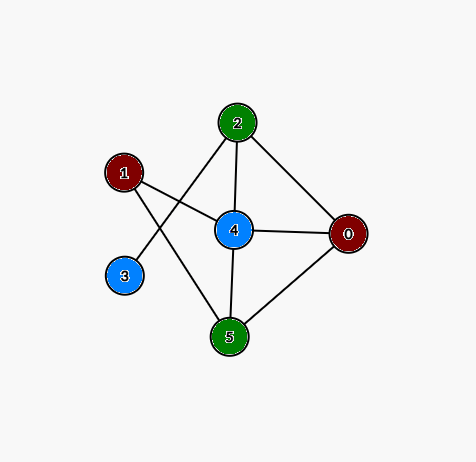
\includegraphics[width=\textwidth]{images/vertex-coloring.png}
      \caption{Vertex coloring}
      \label{fig:vertex-coloring}
  \end{subfigure}
  \hfill
  \begin{subfigure}[b]{0.49\textwidth}
      \centering
      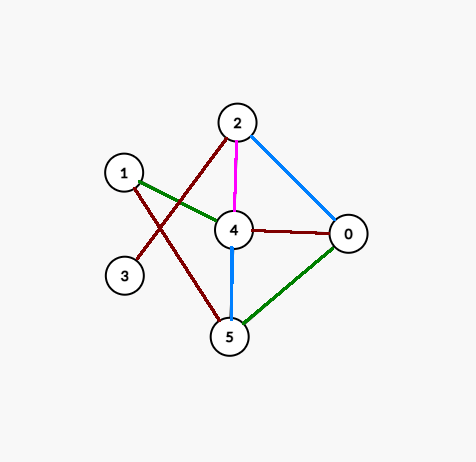
\includegraphics[width=\textwidth]{images/edge-coloring.png}
      \caption{Edge coloring}
      \label{fig:edge-coloring}
  \end{subfigure}

  \hfill
  \begin{subfigure}[b]{0.49\textwidth}
      \centering
      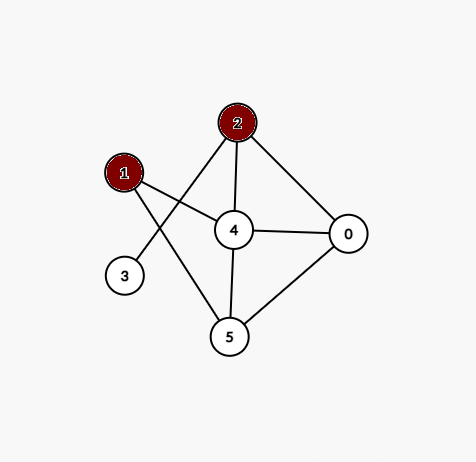
\includegraphics[width=\textwidth]{images/maximal-ind-set.png}
      \caption{Maximal independent set}
      \label{fig:maximal-independent-set}
  \end{subfigure}
  \hfill
  \begin{subfigure}[b]{0.49\textwidth}
      \centering
      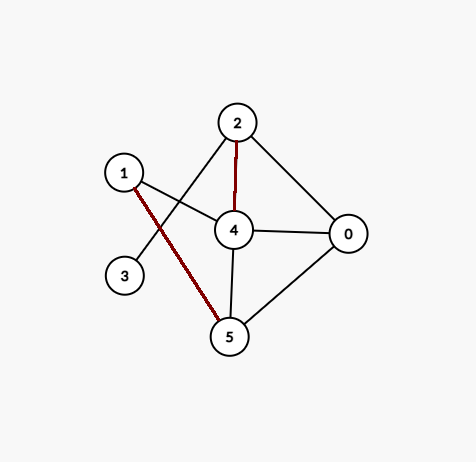
\includegraphics[width=\textwidth]{images/maximal-matching.png}
      \caption{Maximal matching}
      \label{fig:maximal-matching}
  \end{subfigure}
  \caption{Some of the common LCL problems}
  \label{fig:graph-problems}
\end{figure}

Finally, a \textbf{maximal matching problem} is a problem in which nodes need to
produce a matching such that each node is either matched with one of 
its neighbors or it cannot be matched because all of its neighbors are
matched. That is, no node can be left unmatched while at least one of its
neighbors is unmatched. It is trivial to see that the problem is an LCL
since each node can check its radius-1 neighborhood to check whether it
is matched with a neighbor or all neighbors are matched with someone else.
And if the condition of the previous sentence is not satisfied, the output
is invalid.
Refer to Figure~\ref{fig:maximal-matching}, for a
solved instance of the maximal matching problem.

\section{Decidability and undecidability}

Before moving forward, it is important to remind about a notion of
decidability in the context of theoretical computer science. It is
assumed that the reader already has some basic knowledge of
complexity theory, computability, Turing machines, automata, and
languages. The content of this section follows
the definitions and formalisms as defined in the book by Sipser~\cite{Sipser2012}
unless specified otherwise.

First of all, recall that a deterministic Turing machine is called
\emph{decider} if it halts on all inputs. Similarly,
a nondeterministic Turing machine is called a decider, if
it ends up in a halting state in all of its branches. We then
call a language \emph{decidable} if and only if there is some Turing
machine that decides it. That is, a language $L$ is decidable
if and only if there exists some Turing machine $M$ such that given
an input $x$, where $x \in L$, it always halts.

\emph{A decision problem} is an algorithmic problem that has only two
valid solutions to it: ``yes'' and ``no''. We assume that a decision
problem has an infinite set of inputs. That is, a decision problem
defines an infinite but possibly restricted set of valid inputs,
and for each input, only one of the two outputs is the correct
output. An algorithm is said to solve a problem $P$ if and only
if, given any input from a set of valid inputs, it can
always produce the correct output. Recall also that we can
represent any decision problem $P$ as a formal language $L_P$, where
a string $x \in L_P$ if and only if, given that $x$ is an input
to the problem $P$, the correct output is ``yes''. To clarify,
for each problem $P$, there is a language $L_P$ such that
if $P$'s output on some input $x$ is ``yes'', then $x \in L_P$,
otherwise $x \notin L_P$. From now on, I will call such
language $L_P$ that ``represents'' a decision problem $P_L$ as
\emph{corresponding language} of problem $P$.

Then, a decision problem $P$ is \emph{decidable}, if and only if
there is a decidable corresponding language $L_P$.
On the other hand, a decision problem is \emph{undecidable},
if and only if, there is no decidable corresponding language $L_P$.
Note that a problem is undecidable if and only if it is not
decidable.

To prove that a problem $P$ is decidable, it is sufficient to
show an algorithm (formally a Turing machine) $A$, such that
$A$ correctly solves the problem for all valid inputs. That is,
such an algorithm $A$ must always halt and must produce the
output ``yes'' if and only if it is the correct output of the
problem $P$ given the input. Thus, proving decidability
requires finding such an algorithm, and then proving
that $A$ always halts and that $A$ is indeed correct.
To prove that a problem is undecidable is however less
trivial. One of the common techniques is to show that
the problem can be reduced to the Halting problem~\cite{Margenstern2000, Turing1937}.

\section{Automated synthesis and classification}

\emph{Automated classification}, broadly speaking, is a problem
where objects of a certain type, which possibly share some
properties in common, are required to be classified into
several, often in-advance known categories automatically,
that is, without or with minimal human supervision.
Due to the recent successes in the field of machine learning,
numerous automated classification problems have been solved,
or at least for many of the problems, significant
progress has been made. In particular, the field of automated classification
of image, sound, and text data
based on deep neural networks -- one of the popular machine learning
techniques that have had multiple breakthroughs in recent years --
had some significant results in the areas of medicine, biology,
agriculture, and many others~\cite{auto-class_Sharma2017,
auto-class_Capizzi2015, auto-class_Ibrahim2018, auto-class_Colonna2016,
auto-class_Winkler2017, auto-class_FabioDelFrate}.

However, automated classification is also possible beyond
the physical media such as images, sounds, etc. For example,
it is often useful to classify abstract problems, e.g.\ mathematical
or computer science problems. Indeed,
Fulton et al.~\cite{class_Fulton} have shown an approach
for automated classification of Sturm-Liouville
problems~\cite{zettl2010sturm}.

\emph{automated synthesis} is a problem of automatically
synthesizing or finding
a solution to a certain problem given a set of constraints and/or
objectives. For example, automated synthesis is fairly common
in the field of electrical engineering, and is commonly
applied when designing analog and digital circuits~\cite{synthesis_,
synthesis_autoAx}. Furthermore, with the recent rise in popularity
of quantum computing, the need has arisen for the design of quantum
circuits. Similar to the classical cases, the synthesis of
quantum circuits has become a popular research direction
with numerous publications on the matter~\cite{synthesis_Khan2017,
synthesis_Meuli2018, synthesis_Miller2003}.

In general, algorithm synthesis in the context of theoretical
computer science is undecidable. However, there are some
research directions in the field of distributed computing and
distributed algorithms, where some forms of automated synthesis and/or
automated problem classifications have led to successful
developments~\cite{Balliu2018, da-synthesis_Rybicki2015,
da-synthesis_Klinkhamer2016,
da-synthesis_Hirvonen2017, da-synthesis_Fathiyeh2015, da-synthesis_Dolev2016,
Chang2017, Brandt2017, da-synthesis_Bloem2016}. Moreover,
the notions of automated synthesis and automated classification are
often interconnected in the context of distributed algorithms.
To demonstrate this, I take an example of a common problem in
a distributed computing: given a problem $\Pi$, we need to
automatically determine its complexity. Assigning a complexity
class to the problem $\Pi$ can be viewed as a classification
problem here. On the other hand, proofs of the type that
demonstrate that $\Pi$ belongs to a certain complexity class
are often constructive in nature. That is, to show that a
problem can be solved in the number of rounds $x$, we
often need to develop an algorithm that solves the problem
in the stated number of rounds. But developing such an algorithm
can potentially be automated, meaning that \emph{automated
algorithm synthesis} can be used. Thus, in the context of
distributed computing, automated algorithm
synthesis and automated problem classification are often two perspectives
on the same thing: determining whether a problem $\Pi$ can be solved
in $x$ rounds or is fundamentally more difficult.

\section{Recent developments in the automated classification of LCL problems}

At this point that the theoretical background has been given, it is
useful to give a background to much more recent developments in the
distributed algorithms research. As the branch of research of
studying LCL problems had been reaching maturity, many focused
on the idea of automated classification of LCL problems. That is,
the question of interest is whether we can create meta-algorithms
that would take the description of an LCL problem as its input
and produce the problem's round complexity as an output.
Figure~\ref{fig:meta-algorithm} conceptually depicts
an example of a meta-algorithm.
This being the core topic of the thesis, it is thus important
to describe all the prior work done in this direction.
In the rest of the
section, I will introduce some of the negative as well as positive results
related to the automated classification of LCL problems.

The questions of whether a certain family of LCL problems
can be automatically classified are often referred to
as decidability questions. Roughly speaking, a problem is
said to be decidable if there exists an algorithm that,
given the problem, will output its complexity. Such decidability
questions are often studied in relation to the whole
family of graph problems and not to individual instances
of problems.

\begin{figure}[ht]
  \begin{center}
    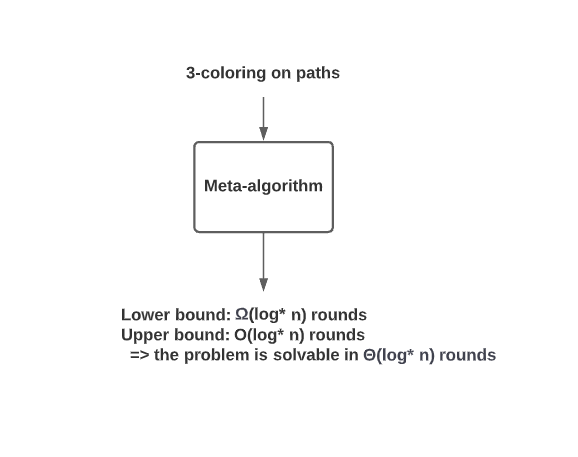
\includegraphics[width=\textwidth]{images/meta-algorithm.png}
    \caption{Conceptual representation of a meta-algorithm}
    \label{fig:meta-algorithm}
  \end{center}
\end{figure}

First of all, it is important to notice that it has been
proven that in general LCL problems are undecidable.
In fact, already in the cases when the graph family is a grid,
LCL problems cannot be automatically classified~\cite{Brandt2017, Naor1993}.

Nevertheless, many interesting LCL problems are still decidable.
For example, it was known for several years now that LCLs
on paths and cycles are decidable~\cite{Balliu2018, Brandt2017, Naor1993}.
Besides, certain types of LCL problems are also decidable on
trees~\cite{Chang2017}.

But the fact that a problem is decidable in theory does not
always imply that it is practical to use an
algorithm for automated classification of
such a problem. For instance, it is known that even in
the case of paths and cycles, if a node labeling is
given as part of the input, decidability becomes
PSPACE hard~\cite{Balliu2018}.

However, not everything looks that gloomy, and many
interesting and sufficiently broad families of LCL
problems are both decidable, and it is feasible to
automatically classify them in practice. Indeed a lot of work
has been done attempting to derive practical algorithms
that determine the complexity of a given LCL problem,
especially in trees.

Balliu et al.~\cite{Balliu2019c} has shown that a complete classification
of binary labeling problems (problems where a node's
output is allowed to be only one of the two possible labels)
at least in a deterministic setting is possible and moreover
can be done in $O(1)$ time since computational
complexity of such problems can be simply looked up in a
table in a constant time. In addition
to this, the paper also shows that it is decidable to
classify at least \emph{some} of the randomized binary labeling
LCL problems~\cite{Balliu2019c}.

Building on top of the work outlined in the paper, Rocher~\cite{Rocher2020clas}
has developed a meta-algorithm that classifies \emph{almost}
all ternary labeling problems on trees in the deterministic
setting. Furthermore,
he also implemented the meta-algorithm as a
computer program written in Python programming language~\cite{Rocher2020doc}.
Although the implementation focuses mainly on the case of trees with degree 3,
the techniques described in the manuscript are applicable to ternary problems
on trees of higher degrees as well.

In addition to this, LCL problems on trees and cycles
are fully decidable in polynomial time as was shown by Chang et al.~\cite{Chang2020}.
The algorithm for classifying the problems can be used in practice and has
been implemented in Python programming language by Aalto's
Distributed Algorithms research group~\cite{Tereshchenko2020}.

Furthermore, a technique called round elimination was introduced in the context
of LCL problems by Brandt et al.~\cite{Brandt2019}. It is a series of mechanical
steps that, if followed, in many cases transform an LCL problem $\Pi_0$ into another LCL problem $\Pi_1$. An interesting property is that, given certain assumptions and the fact that
$\Pi_0$ is solvable in constant time e.g.\ in $T$ rounds, $\Pi_1$ is guaranteed to be
solvable in exactly $T - 1$ rounds. This single property has numerous implications.
For example, if we apply the technique $k$ times and in the end obtain an LCL problem $\Pi_k$
such that it is zero-round solvable, we know that the original problem $\Pi_0$ is
exactly $k$-round solvable. Moreover, round elimination is not only possible
in theory but is also very much feasible in practice.
Indeed, Olivetti~\cite{Olivetti2020} has
implemented a computer program that, given an LCL $\Pi_0$ solvable in $T$ rounds,
it produces another LCL $\Pi_1$ solvable in $T - 1$ rounds. There even exists
a web interface for the program, and one can apply the technique and obtain
its results within milliseconds. I will describe the technique and its implications
in much more detail in the next section.

Finally, very recently, Balliu et al.~\cite{Balliu2021} demonstrated
that LCL problems on rooted trees are completely decidable.
In particular, an LCL problem on rooted trees can be completely
classified in both deterministic and randomized settings. The only
exception to this completeness is deciding whether a given problem
has round complexity of $\Theta(n)$ or it is unsolvable. In addition
to the theoretical results in the manuscript, the authors also
provide a freely available open-source software that can
classify an LCL with a relatively small number of labels in a matter
of milliseconds~\cite{Studeny2021}.
